%************************************************
\section{Black-Box Analysis}\label{ch:Blackbox}
%************************************************
In this section, we introduce the first method we use to analyze configurable software systems, the black-box analysis. 
In \autoref{ch:bb-general-concept}, we explain a black-box and the concepts behind the black-box analysis. 
We proceed in \autoref{section:combinatorial-explosion} to explain the challenges we encounter when using a black-box analysis.
After collecting data, we use them with multiple linear regression to build a performance-influence model in \autoref{ch:linear-regression}.

\subsection{General Concepts}\label{ch:bb-general-concept}

%Introduction why now black-box
We have introduced {\perfInfluenceModel} to represent the influence of each feature and feature interaction on a system. In this section, 
we expand on this topic and introduce the \emph{black-box analysis} a method to collect data to build \perfInfluenceModel.

%What is a black-box and what is the analysis
A black-box of a configurable system is conceptually simple, we execute a given system with a configuration, and after finishing, we receive an output. 
However, the critical part is that we are unaware of how the black-box produces the output. 
Since we cannot see inside the system, we need an approach that does not require this. 
Therefore, in a black-box analysis, we solve this issue by observing the machine on which the system is executed.

\begin{figure}[h]
    \centering
    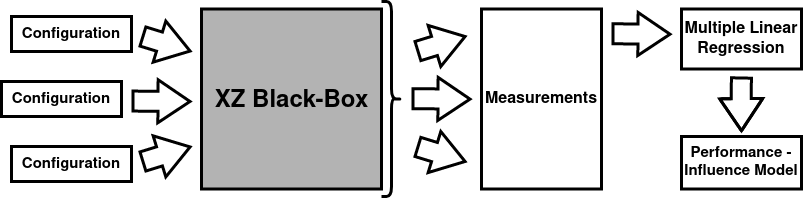
\includegraphics[scale=0.55]{gfx/BlackBox2_0.png}
    \caption{Process of using a black-box analysis to build a \perfInfluenceModel for \textit{XZ}.}
    \label{fig:BBxz}
\end{figure}

%Example of Chapter pipeline
In \autoref{fig:BBxz}, we use a black-box analysis for \textit{XZ} to build a \perfInfluenceModel.
We start by focusing on finding the features that we are interested in. 
Then we build ourselves multiple configurations that hold different interactions between these features.
Afterward, we run \textit{XZ} as a black-box on each configuration; during the execution, we analyze the system by measuring different non-functional properties.
In our case, we are interested in the performance of each feature. 
We repeat this process for each configuration during the black-box analysis and collect the measurements.
Next, we use these measurements together with multiple linear regression to build a \perfInfluenceModel.

\subsubsection{Black-Box Analysis}\label{ch:Black-Box-Analysis}

%Intro in section, combinatorial explosion
Before we start analyzing the system, we first have to select the features we are interested in, since for most configurable systems it is 
not feasible to use the whole configuration space due to its size. This issue is called \emph{combinatorial explosion} in \autoref{section:combinatorial-explosion}
we explain how we deal with this problem.

%The analysis
After deciding which features are of interest to us, we can now turn to the question 
of how we analyze the system and collect the data we need to build a \perfInfluenceModel

As shown in \autoref{fig:BBxz}, we cannot analyze how the system produces the output; 
therefore, we are limited to the non-functional properties we can observe from the outside. For this reason, 
we execute the system with each configuration and measure the property we are interested in, such as energy consumption, memory usage, 
and computational resources used.  

\subsection{Challenges}\label{section:combinatorial-explosion}
%Defining combinatorial explosion
One of the larger problems we face when using black-box analysis is the issue of combinatorial explosion, 
which refers to the effect that when features increase linearly, the number of possible configuration
increase exponentially~\cite{Combinatorial-explosion}.

%Explaining exponential groth more in detail
Suppose we have a configurable system where each feature is a binary option.
We also define that in this system, each feature is entirely independent of another
(i.e., the system has no constraints, and selecting or deselecting one feature has no effect on other features).
The number of unique configurations this system can produce is $2^n$, where $2$ refers to the type of feature options allowed,
binary in our case, and $n$ denotes the number of features. 

%Why it is a problem, Example
Here is the problem, because all these different features can interact with each other in different ways, and for very small systems
we can certainly brute-force our way by benchmarking all possible configuration, however this does not scale, and certainly not feasible for 
larger systems. For example, the Linux kernel contains 10`000 different features~\cite{Linux-Kernel}, for reference it is estimated that the universe
contains about $10^{79}$ atoms, which is still less than the number of unique configurations a system with 263 features produces, it is already impossible to use brute-force to analyze
such a system, let alone the Linux kernel.

%How wo overcome it
Hence, we cannot fully explore the entire configuration space and must select a subset representing the system with high accuracy. 
For this purpose, we take advantage of the findings of Xu et al.~\cite{TooManyKnobs}, 
where they have shown that not all features are equally important and that up to 54,1\% of features are rarely set by users. 
We use this information with our domain knowledge to extract the most important features we are interested in.


\subsection{Multiple Linear Regression} \label{ch:linear-regression}
%Section overview
After collecting all our measurements, we use them to build our {\perfInfluenceModel} of the system. 
This section explains the reasoning behind using \emph{multiple linear regression}. 
Afterward, in \autoref{ch:OLS}, we explain \emph{ordinary least squares}, an estimator to calculate the coefficient of each term inside the \perfInfluenceModel. 
While using \emph{ordinary least squares}, we have to handle the problem of \emph{multicollinear features}; we do this in \autoref{ColinearF}. 
To reduce the degree of \emph{multicollinear features} we introduce the \emph{Variance Inflation Factor} in \autoref{ch:vif}.

%Why Multiple limear regression
When building a \perfInfluenceModel from our black-box data we have the requirement that the model needs to be interpretable. While multiple 
methods to predict performance have been introduced, such as neural networks, they lack the interpretability of the model, which on contrary
\emph{multiple linear regression} provides.

To illustrate why interpretability is important lets inspect the following \perfInfluenceModel:

\begin{align*}
    \Pi_1 &= -1000 + 1001 \cdot \textit{Feature\_A} + 1002 \cdot \textit{feature\_B} - 1000 \cdot \textit{Feature\_A} \cdot \textit{feature\_B} \\
    \Pi_2 &= 0 + 1 \cdot \textit{Feature\_A} + 2 \cdot \textit{feature\_B} + 0 \cdot \textit{Feature\_A} \cdot \textit{feature\_B}
\end{align*}

%Example why we need interpretability
Under the condition that either \textit{Feature\_A} or \textit{Feature\_B} needs to be selected, 
$\Pi_1$ and $\Pi_2$ predict for any configuration the same amount of time, however, 
if we take a close look at how $\Pi_1$ assigns the influence of each feature, we can see that this is not interpretable. 
Here $\Pi_1$ assigns to the \textit{Base} feature an influence of -1000 thousand, 
which does not make sense since the time spent in the \textit{Base} feature can not be negative. 
This also leads to $\Pi_1$ assigning unrealistic amounts of time to features or feature interactions. 

We use the following formula for linear regression for matrices ~\cite{Linear-Regression-Performance}:

\begin{align}\label{formula:linReg}
    Y &= \beta_0 + \beta_1 x_1 + \beta_2 x_2 ... \beta_n x_n + \epsilon   \\
    Y &= X \beta + \epsilon \nonumber\\ \nonumber \\ \nonumber
    Y &= \textit{Dependent variable}\\ \nonumber
    X &= \textit{Independent variable}\\ \nonumber
    \beta &= \textit{Regression coefficient}\\ \nonumber
    \epsilon &= \textit{Error} \nonumber
\end{align}

%For what linear reg is used
The model is used to estimate the relationships between the independent variables and the dependent variable.
In our case, $Y$ is a vector with \textit{n}  elements containing the output of our black-box model,
i.e., the measurements for each configuration in our set of configurations $\mathcal{C}$. 

%Exlaining collums of matrix and how they map to our config
Our independent variable $X$ is an $n \times m$ matrix, where $n$ is the number of configurations used, 
and $m$ is the number of features and feature interactions across all configurations. 
To accommodate feature interactions in this linear model, we add a term for each interaction we want to include. 
For example, if we consider the interaction between features $x_i$ and $x_j$ we add the term $\beta_k x_i x_j$. 

%Explaining coecfficient map to feature
We are interested in the values of the coefficients $\beta$, since they quantify the influence of each feature or feature interaction on the whole system. 
In addition, $\beta_0$ denotes the intercept, representing the influence of the base code, 
meaning the part of the code executed regardless of the chosen configuration.

%Splitting of feature interactions
The value of each feature in the matrix is $1$ if the feature is selected or $0$ if it is not selected.  If we have numerical features with $l$ different options, 
we split these features into $l$ binary features and encode them as an alternative group in our feature model.

%Error
All our measurements have a possible error represented by $\epsilon$~\cite{Linear-Regression}.

\subsubsection{Ordinary Least Squares}\label{ch:OLS}
%Why we need ols
Now that we have seen the general formula of multiple linear regression and know what the different components stand for, we still need to figure out 
how to calculate the regression coefficient $\beta$, the values that tell us the influence of each feature. 

%Why OLS works in detail
For this purpose, we use the ordinary least squares estimator, which is optimal for the class of linear unbiased estimators, 
but is unreliable when the independent variables $X$ contains a high degree of multicollinearity, we explain this in detail in \autoref{ColinearF}.
The principal of ordinary least squares is to minimize the sum of the squared residuals, where the residual is the difference between
the predicted value of the estimator and the actual value.~\cite{Linear-Regression}


\begin{figure}[H]
    \centering
    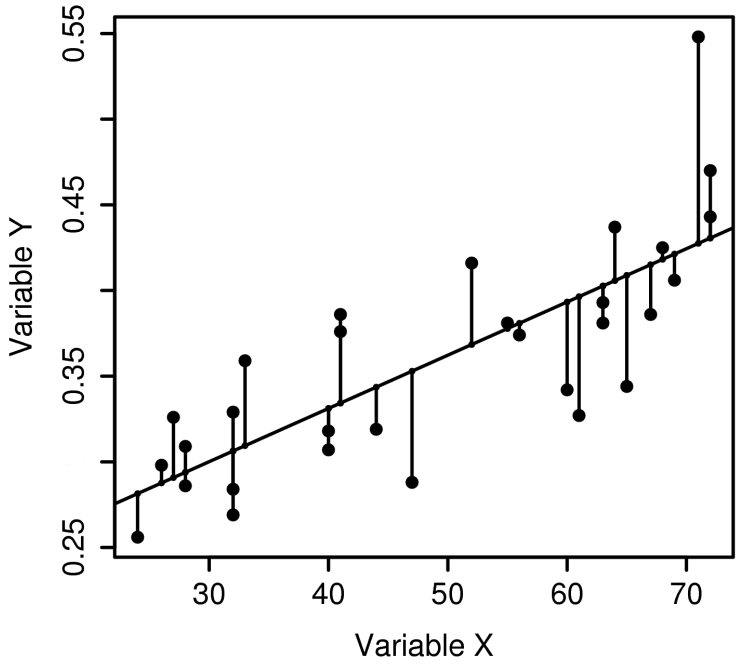
\includegraphics[scale=0.3]{gfx/OLS.png}
    \caption[Ordinary Least Squares regression model residuals]
    {Ordinary Least Squares regression model residuals
    \footnotemark}
    \label{fig:OLS}
\end{figure}
\footnotetext{Visited at 06.03.2023, \url{https://datajobs.com/data-science-repo/OLS-Regression-[GD-Hutcheson].pdf}}

%example illustration
We see an illustration of an ordinary least squares estimator for a linear regression model in \autoref{fig:OLS}, where we have only one variable 
X and the corresponding measurements Y, allowing us to compute the single regressor for this linear regression model.

To compute the regression coefficients using ordinary least squares, the following formula is used~\cite{Linear-Regression}:

\begin{align}
    \hat{\beta} &=  (\textit{X}^{\top } \textit{X} )^{-1}\textit{X}^{\top} Y \\ \nonumber \\\nonumber
    \hat{\beta} &= \textit{Ordinary Least Squares estimator}\\\nonumber
    \top &= \textit{Matrix Transposed}\nonumber
\end{align}\label{equ:ols}

Now $\hat{\beta}$ contains the regression coefficient we are interested in.

As an example, we can refer to our code from \autoref{lst:performanceExample}
and sample some configurations to build a multiple linear regression model using ordinary least squares.

\begin{table}[H]
    \centering
    \begin{tabular}{rrrrrrrr}
    \hline
    Base & A & B & C & A $\land$ B & A $\land$ C &  & $\bm{\Pi(*)}$ \\ \hline
    1    & 0 & 0 & 0 & 0           & 0           &  &  $\mathbf{1}$   \\
    1    & 1 & 0 & 0 & 0           & 0           &  &  $\mathbf{2}$   \\
    1    & 0 & 1 & 0 & 0           & 0           &  &   $\mathbf{3}$  \\  
    1    & 0 & 0 & 1 & 0           & 0           &  &   $\mathbf{2}$  \\  
    1    & 1 & 1 & 0 & 1           & 0           &  &   $\mathbf{6}$   \\
    1    & 1 & 0 & 1 & 0           & 1           &  &   $\mathbf{3}$  \\  
    1    & 0 & 1 & 1 & 0           & 0           &  &   $\mathbf{4}$  \\  
    1    & 1 & 1 & 1 & 1           & 1           &  &   $\mathbf{7}$  \\ \hline

    \end{tabular}  
    \caption{Configuration samples of \autoref{lst:performanceExample}}
\end{table}

Using the configuration samples from \autoref{tab:alternative} we can now determine $\textit{X}$ and $\textit{Y}$:

\begin{displaymath}
    \textit{X} = 
    \begin{bmatrix} 
        1 & 0 & 0 & 0 & 0 & 0 \\
        1 & 1 & 0 & 0 & 0 & 0 \\
        1 & 0 & 1 & 0 & 0 & 0 \\
        1 & 0 & 0 & 1 & 0 & 0 \\
        1 & 1 & 1 & 0 & 1 & 0 \\
        1 & 1 & 0 & 1 & 0 & 1 \\
        1 & 0 & 1 & 1 & 0 & 0 \\
        1 & 1 & 1 & 1 & 1 & 1 
      \end{bmatrix}
      ,
      \textit{Y} =
      \begin{bmatrix}
        1 \\
        2 \\
        3 \\
        2 \\
        6 \\
        3 \\
        4 \\
        7 
      \end{bmatrix}
\end{displaymath}


Using the ordinary least squares \hyperref[equ:ols]{Equation \ref*{equ:ols}}  we obtain the following results:

\begin{equation}
    \hat{\beta} = 1 + 
    \begin{bmatrix}
        0,00 \\
        1,00 \\
        2,00 \\
        1,00 \\
        2,00 \\
        0,00
    \end{bmatrix}
\end{equation}

All values have been rounded to 2 decimal places. 
We can see that all values have been assigned correctly.

Now we can use the values to create the \perfInfluenceModel:

\begin{equation}\label{equ:performanceExamplePIMBlackBox}
    \Pi = 1 + 1 \cdot c(A) + 2 \cdot c(B) + 1 \cdot c(C) + 2 \cdot c(A) \cdot B + 0 \cdot c(A) \cdot c(C)
\end{equation}

\subsubsection{Multicollinear Features}\label{ColinearF}
%Connection/Explantion why multicolinearty is bad
We already mentioned that ordinary least squares is optimal as long as our configurations do not contain multicollinearity. The reason for that
is in presence of multicollinearity the variance of the estimator inflates, which in result hurts the interpretability of the model.
We call features multicollinear when there exist a near linear dependency between these features, meaning we can nearly represent one feature as a combination
of different features and the feature does only provide a small amount of new information to the system~\cite{Linear-Regression}. If a feature does not provide
any new information to the system, then we speak of perfect multicollinearity.

As an example take a look at a {\perfInfluenceModel} for some the monthly expenses of a student:
\begin{equation*}
    monthly\_expenses = \textit{food} + \textit{take\_out}
\end{equation*}

%Explanation and example for perfect multicolinearity
Now this shows multicollinearity between the features \textit{food} and \textit{take\_out}, since \textit{take\_out} is already present in the cost of \textit{food},
furthermore it is a case of perfect multicollinearity, since the feature does not provide any new information.

One way multicollinearity is introduced into a system is by using alternative groups, since the selection of a feature in the
alternative group can be expressed by the combination of all other feature.~\cite{Multicollinearity}

\begin{table}[h]
    \centering
    \begin{tabular}{llllll}
    \hline
    Base & A & B & C &  & $\bm{\Pi(*)}$ \\ \hline
    1 & 1 & 0 & 0 &  & $\mathbf{5}$  \\
    1 & 0 & 1 & 0 &  & $\mathbf{10}$  \\  
    1 & 0 & 0 & 1 &  & $\mathbf{15}$  \\\hline
    \end{tabular}  
    \caption{Configuration example illustrating multicollinearity in an alternative group.
    Where $\bm{\Pi(*)}$ is the sum of all selected features inside the row}\label{tab:alternative}
\end{table}

%Example alternative group
Now consider the example of \autoref{tab:alternative}, where we see a configuration example that contains multicollinear features due to an alternative group.
The example contains a mandatory \textit{Base} feature and 3 features in an alternative \textit{A}, \textit{B}, and \textit{C}.
Now we can always model the present of a feature in an alternative group due to the absence of other feature, here for feature \textit{C} to be selected, 
\textit{B} and \textit{A} needs to be deselected.

\begin{align*}
    \Pi_0(c) &= 0 + 5 \cdot c(A) + 10\cdot c(B) + 20\cdot c(C) \\
    \Pi_1(c) &= 5 + 10 \cdot c(A) + 5\cdot c(B) + 20\cdot c(C) \\
    \Pi_2(c) &= 8 + 20 \cdot c(A) + 10\cdot c(B) + 7\cdot c(C) \\
\end{align*}

This leads to multiple performance-influcence model that are accurate with respect to the individual measurement, 
but make completely different statements when compared.

\begin{table}[h]
    \centering
    \begin{tabular}{lllllll}
    \hline
    $\Pi$ & Base & A & B & C   & &  $\bm{\Pi(\{Base\})}$   \\ \hline
    $\Pi_0$ & 0 & 5  & 10 & 20 & &  $\mathbf{0}$         \\
    $\Pi_1$ & 5 & 10 & 5  & 20 & &  $\mathbf{5}$         \\  
    $\Pi_2$ & 8 & 20 & 10 & 7  & &  $\mathbf{8}$        \\\hline
    \end{tabular}
    \caption{Performance predictions of \autoref{tab:alternative}}\label{tab:Performance-predictions}
\end{table}

%Explain multicollinearity 
Another way multicollinearity is introduced into the system is to have features that are mandatory or connected by a condition. 
If we have features that are mandatory, we cannot distinguish these features with our black-box analysis because they are always selected
together, and we cannot determine the extent to which each feature influences the system.~\cite{Multicollinearity}

%Multicolinearity with mandatory feature explaining examples before
In \autoref{tab:Performance-predictions}, we can see the predictions each of the 3 \perfInfluenceModel make for the configurations $\{Base\}$. 
Now $\Pi_0$, $\Pi_1$, and $\Pi_2$, assign completely different values to the \textit{Base} feature, which makes it impossible for us, the user,
to identify the correct value. The reason is that both \textit{Base} and a feature of the alternative group are mandatory; 
therefore, we cannot measure one without the presence of the other. 
Hence, the values of \textit{Base} or the alternative group feature can be set in any ratio as long as the sum of the two values equals the measured time.

When we decide on which features to use in our configuration set, we use our domain knowledge of the system to reduce the amount multicollinear
features to a minimum.

%\begin{algorithm}[h]
%    \caption{Equivalence \label{alg:Colinear}}
%    \begin{algorithmic}[1]
%
%    \If{$(c \textit{ and }  \lnot d) or (\lnot c \textit{ and } d)$} 
%        \State $c,d \gets False$
%    \EndIf
%
%    \end{algorithmic}
%    \end{algorithm}
%
%By extending the example code from \hyperref[alg:performanceExample]{Algorithm \ref*{alg:performanceExample}} with an additional condition where $C \equiv D$ holds, 
%so that either C or D can be selected without the other, we insert the code snippet \hyperref[alg:Colinear]{Algorithm \ref*{alg:Colinear}} 
%after \hyperref[alg:code_insertion]{Algorithm \ref*{alg:code_insertion}}.

%Now, if we select a configuration c that contains the features \{\{A\}, \{B\}, \{C\}\} we get multiple {\perfInfluenceModel}s:

%\begin{align*}
%    \Pi_1(c) &= 1 + 1\cdot c(C) + 1 \cdot c(D) + 1\cdot c(C) \cdot c(D) \\
%    \Pi_2(c) &= 1 + 0\cdot c(C) + 0 \cdot c(D) + 3\cdot c(C) \cdot c(D) \\
%    \Pi_3(c) &= 1 + 1\cdot c(C) + 2 \cdot c(D) + 0\cdot c(C) \cdot c(D) \\
%\end{align*}

%In $\Pi_1(c)$ and $\Pi_2(c)$, all features are assigned different values from what we would expect when looking at Algorithm \ref{alg:performanceExample},
%while the \perfInfluenceModel of $\Pi_C(c)$ assigns the expected values.

\subsubsection{Variance Inflation Factor}\label{ch:vif}
In reality, multicollinearity is often unavoidable in configurable systems, when we want to model the influence of a feature interaction between features
\textit{A} and \textit{B} we introduce a term $A \cdot B$, this feature interaction is only selected when feature \textit{A} and \textit{B} are selected. 
Due to that reason we can not remove terms that introduce multicollinearity, however we can remove perfect multicollinear since they do not provide our 
system with new information.

To check for perfect multicollinearity we use the variance inflation factor (VIF), where a VIF factor of $\inf$ indicates
that there is perfect multicollinearity between features of feature interactions~\cite{Multicollinearity}.

We compute the VIF using the following equation:

\begin{align}
    VIF_{j} &= \frac{1}{1 - R^{2}_{j}}  \\ \nonumber\\
    R^{2}_{j} &= 1 - \frac{\sum\limits_{\forall c \in \mathcal{T}} (c(o_j) - \overline{c}(o_j))^2} {\sum\limits_{\forall c \in \mathcal{T}}(c(o_j) - f_j(c \setminus o_j))^2}
\end{align}

Where $\mathcal{T}$ is the trainings set containing \textit{j} features $o_j$. The VIF$_{j}$ can be calculated for each feature by using the coefficient
of determination $R^2$. To do this, we need to calculate $R^{2}_j$ for each feature $o_j$, fitting a linear regression function $f_j$ to predict whether $o_j$
is selected in the configuration $c \setminus o_j$, using all other features as predictors and the overall mean $\overline{c}(o_j)$~\cite{Multicollinearity}.

\subsubsection{Deciding which terms by using VIF}
%Explain we cant just remove all mulitcollinear term, but only those introducing perfect algorithm
Multicollinearity is present in nearly every configurable system. 
Therefore, we cannot simply remove every term that introduces multicollinearity into the {\perfInfluenceModel}. 
Therefore, we need a strategy to determine the terms we must remove. For this, we use the VIF to determine the terms that add no new information, 
meaning the features that introduce perfect multicollinearity. To accomplish this, we use the following algorithm:

\begin{algorithm}
    \caption{Iterative VIF to check for perfect multicollinearity}\label{alg:vif_iterative}
    \begin{algorithmic}[1]
    \State $\textbf{Input: } \textit{Model\_to\_check}$, list containing all the terms we want to check 
    \State $\textbf{Output: } \textit{Current\_model}$, list containing no terms that introduce perfect multicollinearity
    \State $\textit{Current\_model} \gets \textbf{[\;]}$ \textbackslash\textbackslash Initialize empty list
    \State $\textit{Current\_model.add(Model\_to\_check.pop())} $ \label{alg:vif_add_item}
    \For{$\textit{Term}\;\textbf{in}\;\textit{Model\_to\_check}$} 
        \State $\textit{Current\_model.add(Term)}$
        \If{$\infty\;\textbf{in}\;\textit{VIF(Current\_model)}$}\label{alg:vif_check} \\    
            \qquad$\textit{Current\_model.remove(Terms)}$ 
        \EndIf
    \EndFor
    \State\Return $\textit{Current\_model}$

    \end{algorithmic}
\end{algorithm}

%Explaining Algortihm
In \refAlgorithm{alg:vif_iterative}, we introduce an algorithm that removes all terms that add multicollinearity to our {\perfInfluenceModel}. 
The algorithm takes as an input $\textit{Model\_to\_check}$ a model with all the terms we want to check for multicollinearity. 
Afterward, for each $\textit{Term}$ in $\textit{Model\_to\_check}$, 
we add $\textit{Term}$ to our $\textit{Current\_model}$ and check in \autorefLine{alg:vif_check} if the term introduced multicollinearity, 
which happens if one VIF value is $\inf$, if this happens we remove $\textit{Term}$ from our $\textit{Current\_model}$. 
In the end, we return $\textit{Current\_model}$, containing all terms that do not introduce multicollinearity.

\mycomment{
    Ich würde es alles ein wenig anders strukturieren. Das sollte ohne großen inhaltlichen Mehraufwand recht simpel sein:
1. Introduction
1.1 Context/Motivation
1.2 Goals
1.3 Contributions
2. Background
2.1 Configurable Systems
2.1.1 General Concepts
2.1.2 Features and Configs
2.1.3 Functional/Non-Function Properties
2.2 Modelling Configurable Systems
2.2.1 Feature Models
2.2.2 Feature Diagrams
-> Ggf. auch keine Einteilung in explizite Unterpunkte für 2.2
2.3 Analyzing Configurable Systems
  -> Das ist dein aktuelles 2.5, da ggf. am Ende noch einen kurzen Absatz, welche Analysemöglichkeiten es gibt (BB/WB) aber detaillierte Beschreibung erfolgt in den Unterkapiteln dazu
2.4 Black-Box-Analysis
2.4.1 General Concepts
2.4.2 Challenges (Aktuell 2.6.1.1)
2.4.3 Multiple Linear Regression (Aktuell 2.6.2)
2.5 White-Box Analysis
2.5.1 General Concepts 
  -> Sollte im Endeffekt, beinhalten was du vor 2.7.1 aktuell hast + 2.7.1 + kurzer Anriss, was Feature Taints sind
2.5.2 VaRA
  -> Das was du auch aktuell zu VaRA hast. Die Unterteilung in Unterkapitel ist hilfreich, aber mMn auch nicht zwangsweise notwendig
}